\section{Introducción}

 En todo trabajo es normal comenzar cada capítulo con una sección de
 introducción donde se describa lo que se va a mostrar en este
 capitulo.Como en la tesis, es más fácil hacer esta sección al final
 del capitulo.

 \section{Que poner}

 \subsection{Numero de capítulos}

 Los capítulos que sean necesarios.Normalmente es mejor poner
 capítulos que describan el estado del arte, y las bases de lo que
 se usó en el desarrollo de la tesis. En estos capítulos, no se
 presentan ideas nuevas o desarrollos propios, solo lo que ya
 estaba. Es una especie de revisión bibliográfica.

 En los capítulos subsecuentes, lo normal es ser muy específico y
 desarrollar con detalle el trabajo realizado, tanto si es
 desarrollo tecnológico como si es en simulación o en experimentación
 real. Estos capítulos suelen ser relativamente cortos y con muchas
 imágenes, gráficas y tablas.

 \subsection{Otras cosas}

 Para poner cosas es bueno basarse en formatos ya preestablecidos.
 La notación de las tablas va antes de la tabla, mientras que la de
 las figuras va abajo. Siempre que se muestra una figura o una tabla
 hay que comentarla en el texto tal como la tabla (\ref{Ta:primer ejemplo2})



\begin{table}
  \centering
  \caption{Tabla de muestra para la tesis}
  \label{Ta:primer ejemplo2}
  \begin{tabular}{|l|c|r|}
    \hline
    % after \\: \hline or \cline{col1-col2} \cline{col3-col4} ...
    Texto & Formulas & Numero \\
    \hline\hline
    Cosa & $\sqrt{x^2 + b^2}$ & 3.1416 \\
    Pasto & $3.2 + e^{-t}$ & 4578 \\
    \hline
  \end{tabular}
\end{table}


\subsection{Mas cosas pa poner}

Pues en este caso solo se agrega una figura. Es importante ver que
para que el documento se mantenga ordenado se ponen las figuras en
un subdirectorio figuras y se llaman desde ahí.

\begin{figure}
	\centering
	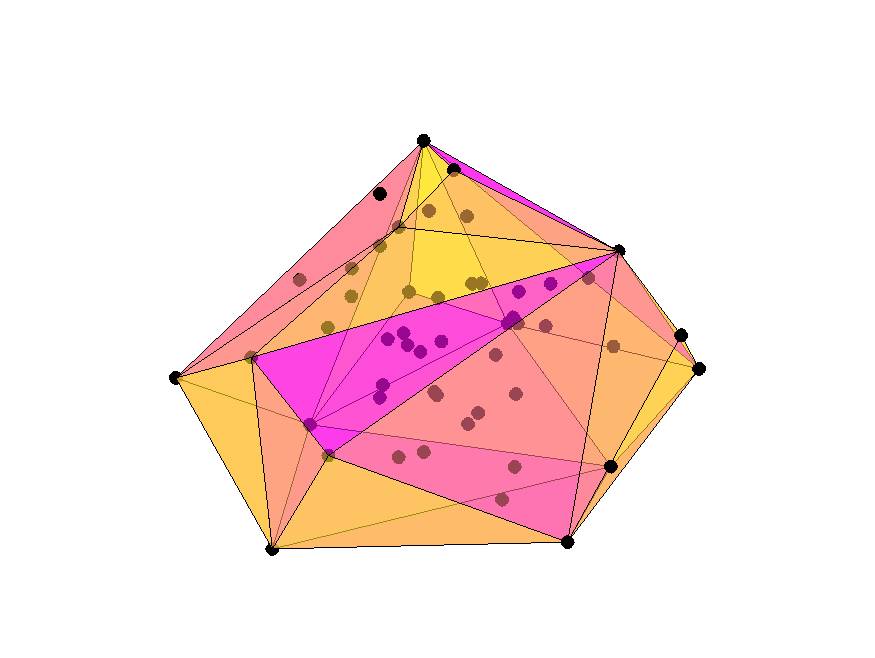
\includegraphics[width=.7\textwidth]{tesislcc/tesela.pdf}
    \caption{Ejemplo de una figura pa la tesis}
    \label{fig:teselacion}
\end{figure}

y bueno pues con esto creo que vemos en general como hacerle en
grandes lineas.

\section{Conclusiones}
En algunos casos no es nada mala idea poner una última sección con
conclusiones de lo que se mostró en el capítulo. 
